\documentclass[border=3pt]{standalone}
% Preâmbulo compartilhado pelos diagramas TikZ da aula 11 (Localização por Grade e Monte Carlo)
\usepackage[T1]{fontenc}
\usepackage[utf8]{inputenc}
\usepackage{lmodern}
\usepackage{amsmath}
\usepackage{xcolor}
\usepackage{tikz}
\usetikzlibrary{arrows.meta,angles,quotes,decorations.pathmorphing,calc,
                positioning,shapes.geometric,shapes.misc,backgrounds,fit,
                math}

% Paleta (mesma dos SVGs originais)
\definecolor{dblue}{HTML}{2A5B8C}
\definecolor{dorange}{HTML}{B3541E}
\definecolor{dgreen}{HTML}{4A7C59}
\definecolor{dred}{HTML}{9C4B4B}
\definecolor{dcream}{HTML}{F4F1EA}
\definecolor{dshade}{HTML}{DDD7C9}

% Função gaussiana (não normalizada por padrão de escala visual)
\pgfmathdeclarefunction{gauss}{3}{%
  \pgfmathparse{1/(#3*sqrt(2*pi))*exp(-((#1-#2)^2)/(2*#3^2))}%
}

% Estilos comuns (prefixo d... para não colidir com chaves internas do pgf)
\tikzset{
  >={Stealth[length=2mm]},
  dguide/.style={gray!55, dashed, line width=0.4pt},
  daxis/.style={gray!60, line width=0.7pt, ->},
  dbody/.style={fill=black!3, draw=black!80, line width=1pt},
  dacc/.style={draw=dblue, line width=1pt},
  dlbl/.style={black!55, font=\small},
  dsub/.style={black!45, font=\footnotesize},
  dstate/.style={circle, draw=black!80, fill=dcream, line width=1pt,
                 minimum size=17mm, font=\large, inner sep=1pt},
  dobs/.style={circle, draw=black!80, fill=dshade, line width=1pt,
               minimum size=14mm, font=\large, inner sep=1pt},
  dbox/.style={rounded corners=2pt, draw=black!80, fill=dcream, line width=1pt,
               align=center, inner sep=6pt},
  dop/.style={circle, draw=black!80, fill=white, line width=1pt,
              minimum size=6mm, inner sep=0pt, font=\small},
  dtrans/.style={->, dblue, line width=1pt},
  dmeas/.style={->, dorange, line width=1pt},
  dcurve/.style={line width=1pt, dblue},
  dcurveb/.style={line width=1.4pt, dorange},
}

\begin{document}
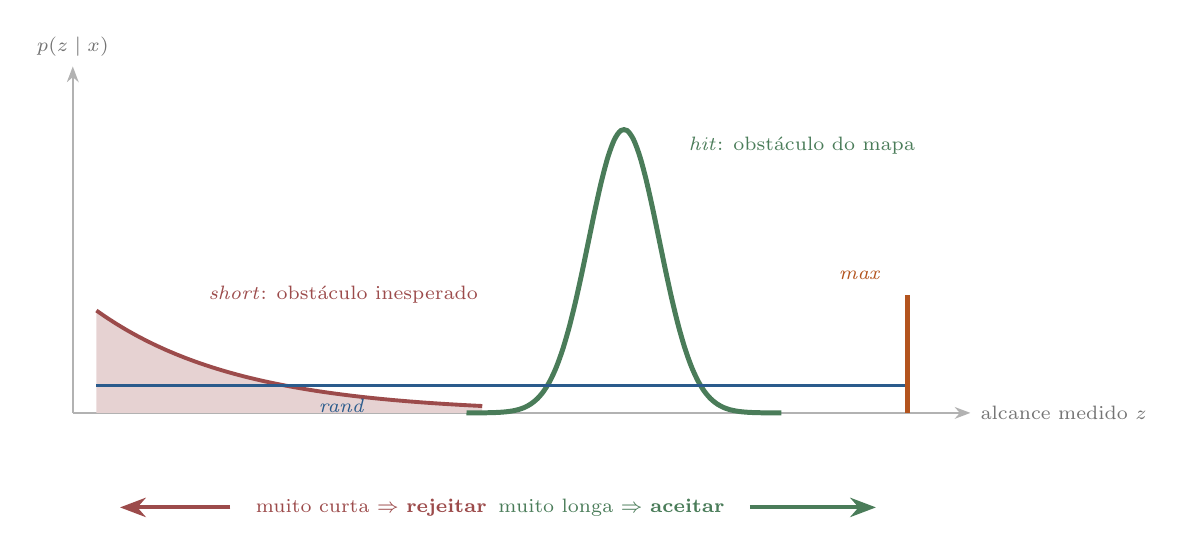
\begin{tikzpicture}[x=1cm,y=1cm]
  \draw[daxis] (0,0) -- (11.4,0) node[right, dlbl, font=\scriptsize] {alcance medido $z$};
  \draw[daxis] (0,0) -- (0,4.4) node[above, dlbl, font=\scriptsize] {$p(z \mid x)$};
  % curta (exponencial)
  \fill[dred!25] (0.3,0) -- plot[domain=0.3:5.2, samples=40] (\x, {1.3*exp(-0.55*(\x-0.3))}) -- (5.2,0) -- cycle;
  \draw[dred, line width=1.4pt, domain=0.3:5.2, samples=40] plot (\x, {1.3*exp(-0.55*(\x-0.3))});
  % hit (gaussiana)
  \draw[dgreen, line width=1.8pt, domain=5.0:9.0, samples=50, smooth] plot (\x, {3.6*exp(-((\x-7.0)^2)/(2*0.45^2))});
  % rand
  \draw[dblue, line width=1.2pt] (0.3,0.35) -- (10.6,0.35);
  % max
  \draw[dorange, line width=2pt] (10.6,0) -- (10.6,1.5);
  \node[dred, font=\scriptsize, anchor=west] at (1.6,1.5) {\textit{short}: obstáculo inesperado};
  \node[dgreen, font=\scriptsize, anchor=west] at (7.7,3.4) {\textit{hit}: obstáculo do mapa};
  \node[dorange, font=\scriptsize, anchor=east] at (10.4,1.75) {\textit{max}};
  \node[dblue, font=\scriptsize, anchor=north west] at (3.0,0.3) {\textit{rand}};
  \draw[dred, line width=1.4pt, -{Stealth}] (2.0,-1.2) -- (0.6,-1.2); \node[dred, font=\scriptsize, anchor=west] at (2.2,-1.2) {muito curta $\Rightarrow$ \textbf{rejeitar}};
  \draw[dgreen, line width=1.4pt, -{Stealth}] (8.6,-1.2) -- (10.2,-1.2); \node[dgreen, font=\scriptsize, anchor=east] at (8.4,-1.2) {muito longa $\Rightarrow$ \textbf{aceitar}};
\end{tikzpicture}
\end{document}
